\documentclass[tikz,border=5mm]{standalone}
\usepackage{tikz}
\usetikzlibrary{arrows.meta, positioning, shapes.geometric, calc, backgrounds, fit, matrix, patterns, decorations.pathmorphing, shadows}

% --- COLOR DEFINITIONS ---
\definecolor{Garnet}{HTML}{73000A}
\definecolor{CSecondaryRed}{HTML}{CC2E40}
\definecolor{CBlue}{HTML}{466A9F}
\definecolor{CDark}{HTML}{1F414D}
\definecolor{COlive}{HTML}{65780B}
\definecolor{CLime}{HTML}{CED318}
\definecolor{CGold}{HTML}{A49137}
\definecolor{CGrayLight}{HTML}{E5E5E5}
\definecolor{CGrayDark}{HTML}{555555}
\definecolor{CWhite}{HTML}{FFFFFF}
\definecolor{CBlack}{HTML}{000000}

\begin{document}

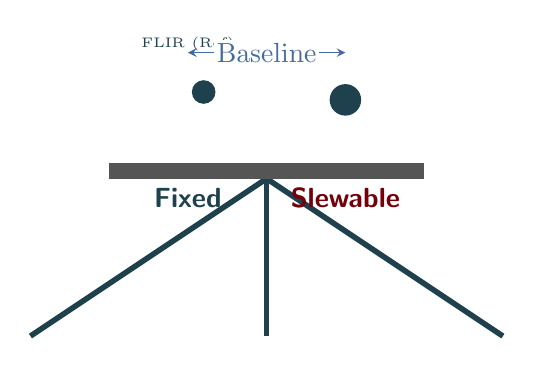
\begin{tikzpicture}
    % Tripod/Mount Base
    \draw[line width=2pt, CDark] (-3, -2) -- (0, 0) -- (3, -2);
    \draw[line width=2pt, CDark] (0, 0) -- (0, -2);
    \fill[CGrayDark] (-2, 0) rectangle (2, 0.2); % Horizontal Bar

    % Camera 1 (Fixed) - Left
    \begin{scope}[shift={(-1, 0.2)}]
        \fill[CWhite] (-0.6, 0) rectangle (0.6, 0.8);
        \fill[CWhite] (0, 0.8) circle (0.5);
        \fill[CDark] (0.2, 0.9) circle (0.15); % Lens
        \node[below, CDark, font=\sffamily\bfseries] at (0, -0.2) {Fixed};
        \node[above, CDark, font=\tiny] at (0, 1.3) {FLIR (Ref)};
    \end{scope}

    % Camera 2 (Slew) - Right
    \begin{scope}[shift={(1, 0.2)}]
        \fill[CWhite] (-0.6, 0) rectangle (0.6, 0.8);
        \fill[CWhite] (0, 0.8) circle (0.5);
        \fill[CDark] (0, 0.8) circle (0.2); % Lens facing front
        \node[below, Garnet, font=\sffamily\bfseries] at (0, -0.2) {Slewable};
    \end{scope}
    
    % Annotations
    \draw[<->, >=stealth, CBlue] (-1, 1.6) -- (1, 1.6) node[midway, fill=white, inner sep=1pt] {Baseline};
\end{tikzpicture}

\end{document}
